% MEng project
% CH1 --- background
%
\documentclass[12pt, a4paper, pdflatex, leqno, twoside, openright]{report}

% Define margins
\usepackage[a4paper,inner=40mm,outer=20mm,top=20mm,bottom=25mm,pdftex]{geometry}

\usepackage[T1]{fontenc} % polsih

% Harvard citation
\usepackage[square]{natbib}
\usepackage{cite} % BiTeX

\usepackage{graphicx}
\usepackage{caption}
\usepackage{subcaption}
\usepackage{url}
\usepackage{listings}
\usepackage{minted}
\definecolor{Bkgd}{rgb}{0.98,0.98,0.98}

\usepackage{datetime}
\newdateformat{monthyeardate}{%
  \monthname[\THEMONTH] \THEYEAR}

% New commands
\newcommand{\ts}{\textsuperscript}
\newcommand{\HRule}{\rule{\linewidth}{0.5mm}}

\newenvironment{dedication}
  {\clearpage               % we want a new page
   \thispagestyle{empty}    % no header and footer
   \vspace*{\stretch{1}}    % some space at the top 
   \itshape                 % the text is in italics
   % \raggedleft            % flush to the right margin
   \raggedright             % flush to the right margin
   \par\setlength{\leftskip}{0.3\textwidth}\noindent\ignorespaces
  }
  {\par                     % end the paragraph
   \vspace{\stretch{3}}     % space at bottom is three times that at the top
   \clearpage               % finish off the page
  }

\usepackage{lipsum}

\usepackage{amsmath}
\usepackage{scalerel}
\DeclareMathOperator*{\Bigcdot}{\scalerel*{\cdot}{\bigodot}}

\begin{document}

\begin{titlepage}
  \begin{center}

\includegraphics[width=0.5\textwidth]{gfx/UOB-logo.png}~\\[2.5cm]

\HRule \\[0.4cm]
{\huge \bfseries
  {\Huge Building activity recognition model:}\\[0.1cm]
  learning Prolog rules and extracting features from spatio-temporal data\\[0.4cm]
}
\HRule \\[1.5cm]

    \begin{minipage}{0.4\textwidth}
      \begin{flushleft} \large
\emph{Author:}\\
Kacper B. \textsc{\textbf{Sokol}}
      \end{flushleft}
    \end{minipage}
    \begin{minipage}{0.4\textwidth}
      \begin{flushright} \large
\emph{Supervisor:} \\
Prof.\ Peter \textsc{\textbf{Flach}}
      \end{flushright}
    \end{minipage}

\let\thefootnote\relax\footnote{\hspace*{-1.7em}Level M/7 $|$ COMSM0130---40cp Individual Project}

\vfill % Bottom of the page
{\large \today}
  \end{center}
\end{titlepage}

\newpage
\thispagestyle{empty}
\mbox{}

\newpage
\thispagestyle{empty}
\mbox{}

% Acknowledgement
\begin{center}\textbf{Declaration}\\[1em]\end{center}
This dissertation is submitted to the University of Bristol in accordance with the requirements of the degree of Master of Engineering in the Faculty of Engineering. It has not been submitted for any other degree or diploma of any examining body. Except where specifically acknowledged, it is all the work of the Author.\\[1.5cm]
Kacper B.\ Sokol, \monthyeardate\today

\newpage
\thispagestyle{empty}
\mbox{}

% Abstract
\begin{abstract}
\thispagestyle{empty}
This project describes \texttt{Prolog}'s \emph{Inductive Logic Programming} approach to learn parametrised rules describing \emph{human activities}. To this end, \emph{Activity Recognition Model} is constructed based on both: simulated data and one collected from smart-house installations. Such premises characterise with vast number of sensors monitoring place of interest, therefore, allow for detailed tracking of \emph{atomic actions} that contribute towards more general activities.\\
Constructed model can be then used to analyse output from smart sites, therefore, describe ongoing human activities. Then, the model is extended to facilitate monitoring of multiple people simultaneously e.g.\ multiple occupiers of a flat.\\
Another, application is to discover structure in the data. Identifying dependencies between sensors and constructing new, more informative features is shown. Both approaches aim at improving performance of classification and are compared and contrasted against the currently most popular model in use: conditional random fields.\\
Furthermore, proposed Activity Recognition Model is extended with basic \emph{Narrative Analytics}. Its goal is to transform generated rules to \emph{natural language}, therefore, produce human readable description of monitored activities.\\

To achieve aforementioned goals, signal issues such as noise, errors, and incompleteness among others are addressed. Furthermore, data transformation is presented: expressing sensors output as knowledge facts. Proposed tool helps to present acquired data in a more transparent way mainly for healthcare applications.\\

To build and test proposed framework both SPHERE Project, and Washington State University CASAS datasets are used.



\begin{center}
Keywords: \textbf{Inductive, Logic, Programming, Prolog, Activity, Recognition, Data, Generation, SPHERE}

% \let\thefootnote\relax\footnote{\noindent This publication including source code is available as \texttt{GIT} repository at: \url{https://github.com/So-Cool/cognition}.}
\end{center}
\end{abstract}



\newpage
\thispagestyle{empty}
\mbox{}
\begin{dedication}
``\ldots~On each landing, opposite the lift-shaft, the poster with the enormous face gazed from the wall. It was one of those pictures, which are so contrived that the eyes follow you about when you move. BIG BROTHER IS WATCHING YOU, the caption beneath it ran.~\ldots''\\[1cm]

``\ldots~The telescreen received and transmitted simultaneously. Any sound that Winston made, above the level of a very low whisper, would be picked up by it, moreover, so long as he remained within the field of vision which the metal plaque commanded, he could be seen as well as heard. There was of course no way of knowing whether you were being watched at any given moment. How often, or on what system, the Thought Police plugged in on any individual wire was guesswork. It was even conceivable that they watched everybody all the time. But at any rate they could plug in your wire whenever they wanted to. You had to live did live, from habit that became instinct in the assumption that every sound you made was overheard, and, except in darkness, every movement scrutinized.~\ldots''\\[2cm]

Nineteen Eighty-Four, George Orwell
\end{dedication}


\newpage
\thispagestyle{empty}
\mbox{}

\newpage
\cleardoublepage
\pagenumbering{gobble}
\tableofcontents
\cleardoublepage
\pagenumbering{arabic}

% \newpage
% \thispagestyle{empty}
% \mbox{}

%===============================================================================
%===============================================================================
%===============================================================================
%===============================================================================
%===============================================================================
\chapter{Introduction\label{ch:introduction}} %Background
\setcounter{page}{1}
% -------- plain English -> explain to someone
% Start with motivation - what is the problem and why it's interesting
% SPHERE somewhere here
% and application - what to do with it
% give solution
% then technique - why technique is best for solution - and more technical details
% --------
% What the project will produce -> contribution
% level of technical challenge
% how the output will be assessed - evaluation
% --------

  \section{The activity recognition}
    \subsection{Outline} %Problem outline
The main aim of the project is to build \emph{activity recognition model} for \emph{smart house} monitoring purposes.\\
By the latter I understand a premise that is fitted with variety of sensors like: motion, door, appliances, water, item, etc.; as well as more sophisticated monitoring devices like cameras, and depth cameras. The first kind of sensors generate raw output usually of a form \texttt{sensorID on}/\texttt{sensorID off}, while the latter type outputs complex signal that needs to be pre-processed to be used as an input of classifiers. Due to aforementioned sensor characteristics my work is mainly focus on the first type of sensors.\\
Therefore in presented above scenario, activity recognition model is a set of techniques that applied to real time signals generated by a house produce a prediction of currently held activity like \emph{cooking} or \emph{sleeping} assigned to one of the premise \emph{residents}. The best solution to sketched above problem is one that works in \emph{signal streaming environment} therefore producing real-time activity predictions with high recognition rate.

    \subsection{Motivation} %Problem motivation/Applications
% Why interesting -> it generalises to any spatio-temporal data therefore can be used
Proposed here activity recognition model is a special case of \emph{predictive model} for \emph{spatio-temporal} data. In general such techniques predict quantity of interest based on input data that encode both location and time of the event of interest.\\
% Why is it needed -> spatio-temporal data is everywhere,
This generalisation have wide variety of real-life applications therefore addressing problems defined as ``hard'' in the activity recognition literature would make valuable contribution to the field. 
First and foremost area of application is healthcare.
% Population ageing - society geting older,  SPHERE project

      \subsubsection{Healthcare: The SPHERE Project}
Allowing elderly people and clinical patients to live at home regardless of health conditions they suffer greatly benefits such individuals. Dwelling in cosy environment causes less stress and individuals being located at home means no need for specialistic day care centres and less crowded hospitals.\\
Therefore, being able to monitor behaviour of people in their own houses and effectively describe their activities result in better patient care possibilities. Such methods allow quick response to any kind of incidents without disturbing monitored people when it is unnecessary.

\begin{figure}
  \centering
  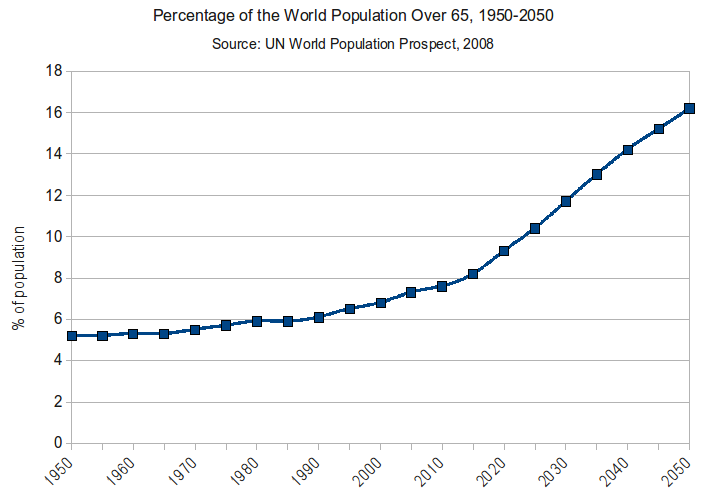
\includegraphics[scale=.5]{./gfx/populationOver65}
  \caption{Percentage of world population over 65, 1950--2050; \citep{populationAgeing}.\label{fig:agingPopulatiom}}
\end{figure}

% The Challenge
The problems of ageing population (see \emph{Figure~\ref{fig:agingPopulatiom}}), global population health issues, increasing healthcare costs, and decreasing quality of life are addressed by the \emph{SPHERE Project} hosted at the University of Bristol \citep{sphere}. This collaboration of clinicians, engineers, designers, social care professionals and various members of the public develops helpful technologies addressing real healthcare problems in a cost effective way.\\
The project focuses on developing real-world technologies which are acceptable in people's homes i.e.\ do not hindering everyday-life. SPHERE works on both hardware and software smart house solutions: sensors and wearable devices as well as algorithms for healthcare applications. The first, are fitted in the place of interest to monitor it and generate various kind of signals, while the latter, use acquired information to identify medical or well-being issues: predict falls, detect strokes, analyse eating behaviour, and detect periods of depression or anxiety.\\
This project extends algorithmic part of undertaken by SPHERE research by proposing novel data analysis framework.

      \subsubsection{Smart City}
Despite huge popularity in healthcare, spatio-temporal data feeds can also be found in variety of monitoring applications. One of them described by \citet{filipponi2010smart} is smart-city management. Automatic analysis---quick and robust---of traffic information, accident reports, etc.\ is of invaluable help in case of emergency.\\
Among many possible applications, produced analysis can result in timely police intervention or well planned route for emergency services, therefore, help in evacuation, crowd management, terrorist attack prevention and airport security control.

      \subsubsection{Complex Systems}
Spatio-temporal data are also produced in large quantities by many of complex systems monitoring and control devices, e.g.: scientific facilities, buildings, data centres~\citep{moore2005data} and power plants~\citep{amin2005toward}. 
Tasks impossible to handle by humans either due to large data volume throughput or demand for low response time are vast area of application for spatio-temporal data analysis. Such tools facilitate well suited for needs system management and risk detection. Power distribution and balancing, nuclear reactor control, data centre heat management are such tasks to name a few.

      \subsubsection{Wildlife}
Monitoring animals behaviour in their natural habitat is an important source of information for many researchers~\citep{Szewczyk:2004:HMS:990680.990704}. Nevertheless, this task is very often impractical either due to adverse climate or difficult access to monitored place. Moreover, scientists in many cases want to avoid disturbing animals' life-cycle and habitats. Difficult access to such sites can be easily overcome with wide range of available sensors and analytic tools, which share common ground with activity recognition model.


  \section{Contribution}
    \subsection{Existing work}
Over the last few years, building machine learning models for \emph{Activity of Daily Living} (ADL) has become an interest of many researchers. Its wide area of applications and increasing complexity appearing with every new discovery attracts now and then machine learning community with new and innovating ideas.\\

    \subsubsection{Techniques}
Up to date, extensive work on houses occupied with both \emph{single}~\citep{cook2009assessing,fatima2013unified} and \emph{multiple}~\citep{hsu2010strategies,singla2010recognizing,crandall2009coping} residents has been done, nevertheless, vast majority focused on state-of-the-art learning algorithm such as:
\begin{itemize}
\item transfer learning---\citet{cook2013transfer},
\item conditional random field---\citet{hsu2010strategies,van2010activity},
\item support vector machines with various kernels---\citet{fatima2013unified},
\item hidden Markov model---\citet{rashidi2011discovering},
\item na\"{\i}ve Bayes---\citet{cook2013activity},
\item artificial neural networks---\citet{fatima2013unified,fatima2013analysis}.
\end{itemize}

All of these models are fuelled by variety of features extracted from raw signals by transformation and time manipulation. Majority of undertaken work in this field uses motion sensors as main source for feature construction with little to none attention to item sensors.\\

Unfortunately, scientific environment focuses on mainstream models and forget about possibly simpler and more suitable but less popular techniques. Observing this gap in spatio-temporal data analysis opens vast new area of research of building activity recognition models with less popular machine learning techniques which is addressed in this paper.

      \subsubsection{Datasets}
Training and testing any activity recognition model requires a dataset of recorded human activities. Such data can be only obtained by designing and building a test-bed house fitted with variety of sensors followed by numerous ``plays'' of scripted activities. As majority of researchers cannot invest time or money to construct a smart house they use publicly available datasets generated by one of research facilities. The most popular choice~\citep{fatima2013unified,fatima2013analysis,nazerfard2010conditional,cook2009assessing} among researchers are datasets published by \citet{cook2009assessing} working at \emph{Center for Advanced Studies in Adaptive Systems}, Washington State University; also known as \emph{CASAS datasets}.\\
Their popularity is based on large amount of variety of recorded activities, with both single and multiple occupiers, available publicly free of charge. Furthermore, they are fairly well formatted and documented nevertheless, they sometimes show inconsistency with labelling structure.

      \subsubsection{Issues}
Tasks such as activity recognition aim at predicting nearly infinite amount of human activities which can be performed in variety of manners. This enormous complexity of the task causes numerous problems ranging from activity prediction, to assigning one of multiple occupiers to performed task. Such ``multi layered'' predictions yield many possibilities for assessing performance e.g.\ correct activity, wrong agent prediction; correct activity, correct agent prediction; etc..\\

The literature identifies building model for some of the activities as relatively difficult. Many of them involve complex, time consuming tasks with multiple residents crossing each others paths. Some of them are addressed in latter parts of this work.\\

Finally, due to specific to dataset output formatting and sensor name-space learnt models are not universal.

      \subsubsection{Outcomes}
Outcomes of activity modelling tasks reported in the literature are unfortunately poor reference for assessing model performance. Use of different datasets and fitness measures depending on study make result comparison impractical.\\
For instance,~\citet{fatima2013analysis} report \emph{accuracy} ranging from $\sim0.2$ to $\sim1.0$ depending on model, dataset and predicted activity.


    \subsection{Project contribution}
Broad activity recognition literature and variety of tested therein models clearly indicate that no single classifier can handle diversity of activity structures embedded in the data. Each model has its pros and cons therefore perfect solution should use all of the models offering features not covered by the others---the concept known as \emph{ensemble learning}.\\

As none of published so far piece of literature discusses application of \emph{first-order formulas} i.e.\ parametrised logical rules, as building blocks of activity recognition model this work comprehensibly covers this problem to expand collection of used techniques. Therefore, the main aim of the project is to apply \emph{Inductive Logic Programming} (ILP) techniques to spatio-temporal data acquired from ``smart'' installations---houses in particular---in order to build \emph{Activity Recognition Model} and extract new, more informative features from raw signals.\\

To address the first problem capabilities of ILP system and model description via set of first-order logical rules are investigated. Both cases: houses with single and multiple occupiers are examined.\\
The latter task involves critical analysis of designed for model learning signal features and assessing their quality. Such novel signal characteristics can be used in any other activity recognition model to boost its performance.\\

Designing a new model and signal features can become difficult task when exact structure of used dataset is unknown. Therefore, systematic way of \emph{generating smart-house data} within user controlled environment is desirable. As part of this project highly customisable data generator is proposed. Such tool facilitates generating datasets representing activities of arbitrary complexity therefore produced data can be used to build and test activity recognition models in (in)deterministic world simulation. Moreover, produced by the generator datasets are invaluable help to systematically compare and contrasting all the learning methods.\\

Finally, the project aims at proposing \emph{unified activity-recognition model evaluation measures}. A systematic way of assessing performance of classifier in activity recognition tasks is beneficial for comparing and contrasting multiple solutions. With such techniques unambiguous assessment of multiple methods for particular activity is possible yielding obvious identification of best solution.

\section{Techniques}
To achieve set above goals performance of proposed technique is evaluate on both \emph{CASAS datasets} and \emph{CASAS-inspired synthetic} datasets produced by the generator. Both datasets are translated from log-like format into \emph{knowledge representation} i.e.\ sensor readings are expressed as logical facts. The evaluation is made by means of \emph{cross-validation}. CASAS datasets are split into activities per person to produce folds so that each fold contains number of activities performed by single person. On the other hand, when evaluating synthetic data each fold is generated independently with common activity structure and small variation of order of used items and detours from originally planned motion trajectory.\\

% why I think it's best for the problem -> more details
The core of proposed technique is \texttt{ALEPH}---Inductive Logic Programming system producing \texttt{Prolog} clauses as the model of data. This approach to learning activity recognition model was chosen as it lacks needed attention in the subject literature.\\

Proposed here rule based classifier greatly differs from currently used methods. Instead of employing \emph{propositional logic} it uses more powerful first-order logic, to express data and activity structure believes. More advanced ``grammar'' implies more possibilities to express complex relations between sensor events. This extra power can be harnessed to compose new data features which can be used in training other models and potentially improve their performance.\\

Furthermore, expressing the activity model in \texttt{Prolog} programming language brings to power all its advantages. Easy \emph{search space traversal} and built-in \emph{failure by negation} are invaluable tools in feature construction. Finally, learnt activity recognition model can be easily transformed to a \emph{generative model} for data hence, serve as an activity example generator.\\
\texttt{Prolog} is also well known for its \emph{natural language processing} capabilities. Rule based model can be therefore used to produce \emph{Data Narrative}---a plain English interpretation of the data which supersedes any other visualisation technique targeted at general public.\\

Another advantage of ILP learning is use of \emph{background knowledge}. It encodes \emph{clauses} needed to build the target model but can also contain any information or rules that might be beneficial for raw data interaction.\\
In smart-house model such component is of invaluable help as it can contain all the house and activity details that are absent in raw data. Room layout, sensor placement, activity structure are just some of them.\\
Moreover, background knowledge acts as a \emph{proxy} between raw data and model, making the latter universal. It means that in majority of cases model learnt for one dataset can be applied to any other by using data-specific background knowledge.\\

Very often monitored activities exhibit hierarchy and structure. Rule based model allow to easily adjust the \emph{resolution of prediction} therefore, activities can be described with different level of depth. Considering activity of eating, the model can simply predict the activity: \emph{eating}; it can also suggest meal type (breakfast, lunch, brunch, etc.) based on time of day; or even food type (pasta, pizza, etc.) based on used ingredients.\\

Rule based model has one more distinctive feature not exhibited by many other machine learning models: it is \emph{human readable}. Such models are easy to inspect and tune simply by eye-balling. Rules can be evaluated whether they make sense, obscure information can be discover and gained knowledge used to design new more suitable features in iterative manner. Rule manipulation is also feasible therefore, they can be simplified (by removing predicate), extended (by appending predicate), or combined (by enclosing them in meta-rule).\\

\section{Deliverables}
% Deliverables / contribution -> what the project will result in
The project delivers highly customizable smart-house data generator written in \texttt{Python}. It is publicly available as a \texttt{GitHub} repository\footnote{\noindent\url{https://github.com/So-Cool/SHgen}} to help researchers with training and testing models.\\
The smart-house simulator is highly customisable: room layout, motion and item sensor placement, and number of occupiers can be specified. The user specifies \emph{action script} which is then ``played'' by house occupiers what in turn produces sensor activations which are recorded in CASAS-like format.\\
As all the actions are ``directed'' precise \emph{ground truth} information is available. Presence of \emph{activity labels} in the data and precise control over the sensor interactions is of invaluable help in experiments of this kind. Finally, the data generator is proved to produces real-like data therefore it is sound for use in model creation and evaluation.\\
The generator repository contains detailed design and usage description to be easy to set-up and use for anybody. The choice of programming language was made based on its popularity making contribution, maintenance and development easy for whole community.\\

Moreover, the project studies in great detail application of ILP to various smart-house settings. Signal output as knowledge representation is proposed. Activity recognition problems defined in literature as ``hard'' for both single and multiple residents are attempted and quality of results is discussed. The capabilities, limitations and advantages of ILP in described scenario is thoroughly investigated and illustrated with examples. The role of background knowledge encoding additional signal characteristics is examined. Used signal features are described and their role in model construction is critically evaluated. Finally, result evaluation techniques are proposed and used to score achieved results.

\section{Challenges}
Issues in all layers: data, ILP and result evaluation arise. To overcome them, multiple solutions are presented and tested to select the best possible one for smart-house data analysis.\\

% prediction continuity issues, and readings in time continuity issues
Very often the data collected from smart-houses are corrupted or obscure due to incompleteness and sensor noise. This phenomenon leads to confusing gaps between ``observed'' actions causing model learning difficulties and intermittent prediction space. With help of inductive learning such implicit information---describing intermediate steps between actions---can be inferred to overcome rule creation difficulty and produce logically consistent scenario.\\
Moreover output of smart-house installations is an unlabelled dataset. Filling the missing activity description is manual labour hence it is time consuming and prone to errors. Lack of reliable ground truth information very often causes model learning difficulties.\\

First-order logic data representation has many advantages but it struggles with unbounded variables like real numbers. This drawback imposes limitations on time and real-valued sensor output representation which is crucial for spatio-temporal data. Discovering possible representations and evaluating their usefulness is of great importance.\\

Learning a data model with ILP is a complex process with number of intermediate steps. First, the learning environment of \texttt{Aleph} ILP system has to be configured to build activity recognition model. For this purpose variety of activity rule structures has to be discovered. Then, datasets and activity scripts need to be analysed to find any relevant structures to extract and format them as signal features. To this end, mechanism in form of \texttt{Prolog} rules has to be built.\\
Background knowledge---the main component of \texttt{Aleph}---is a powerful tool. To make the best use of it, its capabilities and limitations must be discovered. Deciding on useful for feature construction information not contained in the original dataset like room and sensor layout is necessary.\\

Adjusting the resolution (level of detail) of achieved prediction is also a significant task. Therefore, right balance in prediction detail and accuracy trade-off has to be found.\\
Handling data of house occupied by multiple residents introduces difficulty of distinguishing them. Well known problem of agents sharing common space or crossing each other paths has to be resolved.\\

Finally, designing the most suitable an universal evaluation technique is crucial for results comparison. The main difficulty of this task are multiple classification error possibilities. The significance of each of them has to be considered to build performance metric that express real-life usefulness of proposed methodology.

\section{Result evaluation}
For the proposed generator to be publicly accepted in the community dealing with smart-house activity recognition the proof of producing real-like data is necessary. Presented here proof is based on treating output of the generator with model learnt on real data and vice versa. This technique aims at assessing similarity between synthetic and real data.\\

% OUtput asses ->
To prove importance of presented here activity recognition work systematic and versatile evaluation technique is necessary. Firstly, similar technique to generator evaluation is used: applying ``synthetic'' model to genuine data and vice versa. Moreover, different than rule based models are used on both type of data to compare their performance against proposed here technique.\\
Evaluation measures such as accuracy per activity, overall accuracy, accuracy per person per activity are used. Furthermore, for single occupier cases the raw signals are translated into \texttt{ARFF} format and different machine learning models from \texttt{Weka} package are applied to it.\\
Finally, all evaluation is based on \emph{cross validation} to make it more robust. The genuine data is split per person so that each fold contains 5 different activities. The synthetic data is generated with random bits based on script corresponding to the genuine data.


%===============================================================================
%===============================================================================
%===============================================================================
%===============================================================================
%===============================================================================
\chapter{Spatio-temporal data\label{ch:stData}}
Spatio-temporal class of data characterises by entries encoding time and event. Such data are generated by monitoring systems, logs and all kind of smart-instillations like houses and cities. Majority of such datasets occurs in signal streaming scenarios therefore it is implicitly assumed that learning algorithm can look into the past but never see future. This assumption allows to predict current current state based on past prediction. Aforementioned practice is widely used to boost prediction accuracy nevertheless, discussing danger of skewing future predictions by propagating early made error is very often omitted in the studies.

  \section{The data}
My work focuses on smart-house data which is the most popular case of spatio-temporal data. Each entry in such dataset is caused by change of sensor state and is characterised with \emph{time stamp}, \emph{sensor ID} and new \emph{sensor state}.\\
The research world focuses on activity recognition tasks due to many important applications and vast number of activities and their diverse complexity. Hidden in data activities can be very simple or highly complex making model making tasks .\\

but the generalisation of the solution is straight forward --- solution for smart houses can be easly generalised ot other cases.\\
The most popular sensors used in analysed data are: motion, door, item and appliance (fixed-phone, water, hob) sensors.

    \subsection{CASAS dataset}
To ... possible applications of ILP in activity recognition CASAS datasets are used.
very popular
transparent data structure fo given above form
many testbeds 
many played activities
single and multiple occupiers\\

The datasets are structured as a list of sensor readings containing one entry per line of the form: \texttt{Date}---\texttt{Time}---\texttt{SensorID}---\texttt{Value}. Snippets of CASAS dataset is presented in \emph{Listing~\ref{lst:CASASoneR}} for single resident and in \emph{Listing~\ref{lst:CASAStwoR}} for two residents.\\
In both cases 4\ts{th} and 5\ts{th} sparse column is present. Single resident datasets use them to express \emph{activity ID} and \emph{activity status}: ---\texttt{activityID}---\texttt{begin}/\texttt{end}; the latter additionally encodes \emph{resident ID}: ---\texttt{personID\_activityID}---\texttt{begin}/\texttt{end}.

      \subsubsection{Single resident}
The datasets used for model building and testing are ones generated at \emph{Washington State University} as part of \emph{CASAS} project~\citep{cook2009assessing}. \emph{WSU Smart Apartment ADL Normal Testbed} and \emph{WSU Smart Apartment ADL Error Testbed} are the two most popular ones hence are used in the project.\\



% \vspace{1em}
\begin{figure}[htb]
\lstset{
  captionpos=b,
  frame=single,
  backgroundcolor=\color{Bkgd},
  rulecolor=\color{black},
  language=HTML,
  breaklines=true,
  caption=CASAS single occupier dataset structure.,
  label=lst:CASASoneR,
  float=tb
}
  \begin{lstlisting}
...
2008-02-26 10:52:58.577436 M17   OFF
2008-02-26 10:52:59.648222 M18   OFF       cook       begin
2008-02-26 10:52:59.792264 M17   ON
...
2008-02-26 10:53:43.512642 I02   ABSENT
2008-02-26 10:53:43.978491 I01   ABSENT
...
2008-02-26 10:53:52.112690 AD1-B 0.0421491
2008-02-26 10:53:54.721822 M17   ON        phone_call end
2008-02-26 10:53:55.107910 AD1-B 0.155979
...
  \end{lstlisting}
\end{figure}
% \vspace{1em}

The datasets were generated with sensors fitted into living space of house and agents performing predefined activities. The following sensors were used:
\begin{description}
\item[M$\Bigcdot\Bigcdot$] motion sensors;
\item[~I$\Bigcdot\Bigcdot$] item sensors: oatmeal, raisin, brown sugar, bowl, measuring spoon, medicine container, phone book;
\item[D01] cabinet sensor;
\item[AD1-A, AD1-B] water sensor;
\item[AD1-C] burner sensor;
\item[asterisk] phone usage.
\end{description}

The sensor layout of the apartment is shown in the \emph{Figure~\ref{fig:house}}.

\begin{figure}[htb]
  \centering%[width=.45\textwidth]
  \begin{subfigure}[b]{0.6\textwidth}
    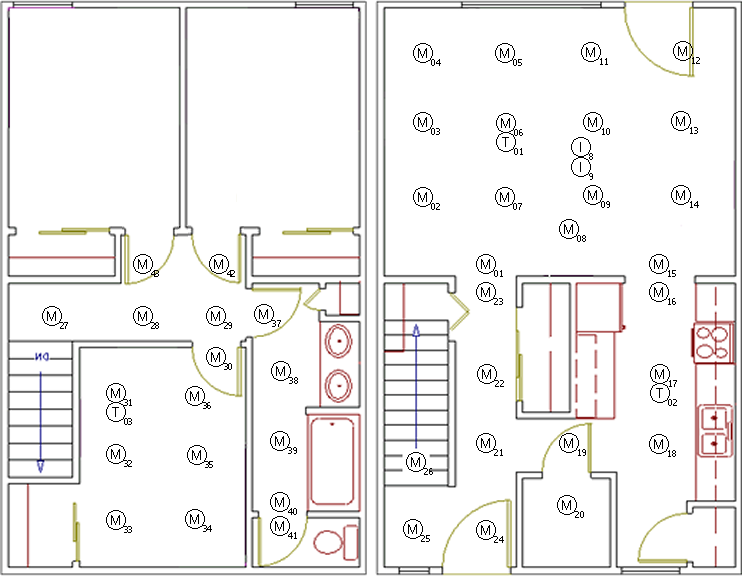
\includegraphics[height=6.3cm]{gfx/Chinook_3_Bedroom_TH}
    \caption{\label{fig:oner:a}}
  \end{subfigure}%
  \begin{subfigure}[b]{0.3\textwidth}
    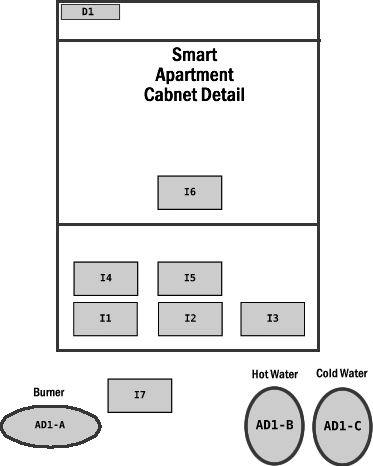
\includegraphics[height=6.3cm]{gfx/Chinook_Cabinet}
    \caption{\label{fig:oner:b}}
  \end{subfigure}%
  \caption[The sensor layout of the apartment.]{The sensor layout of the apartment~\citep{cook2009assessing}.\label{fig:oner}}
\end{figure}

Participants performed five \emph{Activity of Daily Living}(ADL) tasks:
which are scripted!
\begin{description}
\item[Make a phone call] Move to the phone in the dining room; find a specific number in the phone book; dial the number; listens to the message; summarise cooking directions provided over the phone on a notepad.
\item[Wash hands] Move into the kitchen; wash hands in the sink with hand soap; dry hands with a paper towel.
\item[Cook] Cook a pot of oatmeal according to the directions given in the phone message: measure water, pour the water into a pot; boil the water; add oats; put the oatmeal into a bowl; add raisins and brown sugar.
\item[Eat] Take cooked oatmeal; take medicine container; move to the dining room; eat the food.
\item[Clean] Take all of the dishes to the sink in the kitchen; clean them with water and dish soap.
\end{description}


      \subsubsection{Multiple residents}
WSU Smart Apartment 2009 Two Resident Testbed

This dataset represents sensor events collected in the WSU smart apartment testbed during the spring of 2009.  The apartment housed two residents, R1 and R2, at this time and they performed their normal daily activities.

\begin{description}
\item[T$\Bigcdot\Bigcdot$] temperature sensors;
\item[P001] electricity usage.
\end{description}

additionally: $\Bigcdot$ R1 R2
\begin{itemize}
\item Clean
\item Meal\_Preparation  
\item R$\Bigcdot$\_Bed\_to\_Toilet
\item R$\Bigcdot$\_Personal\_Hygiene
\item R$\Bigcdot$\_Sleep
\item R$\Bigcdot$\_Work
\item Study
\item Wash\_Bathtub
\item Watch\_TV
\end{itemize}

\begin{figure}[htb]
  \centering%[width=.45\textwidth] % [height=6.3cm]
  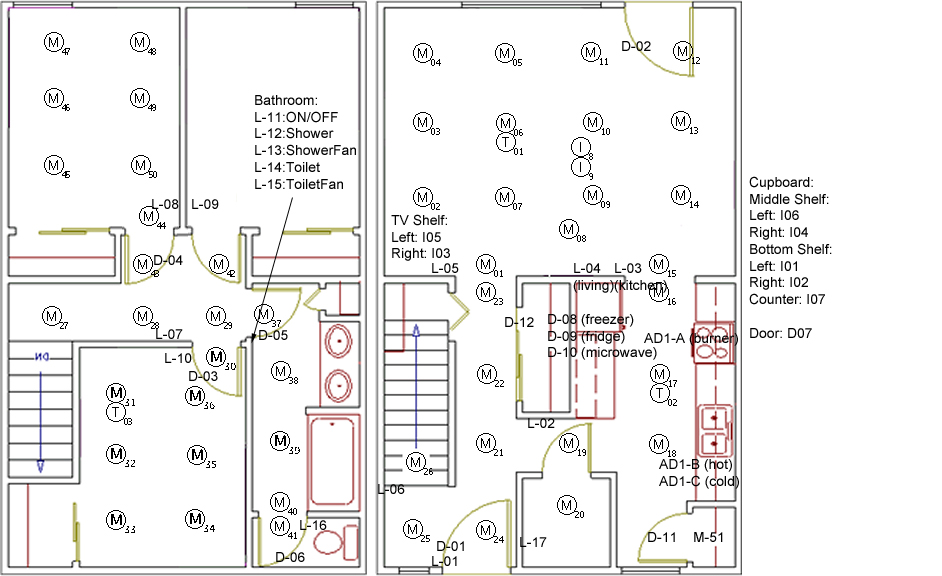
\includegraphics[height=6.3cm]{gfx/sensorlayoutTWOR.jpg}
  \caption[Two residents test-bed sensor layout.]{Two residents test-bed sensor layout~\citep{cook2009assessing}.\label{fig:twor}}
\end{figure}

For multi-occupier case ... is used which looks like

% \vspace{1em}
\begin{figure}[htb]
\lstset{
  captionpos=b,
  frame=single,
  backgroundcolor=\color{Bkgd},
  rulecolor=\color{black},
  language=HTML,
  breaklines=true,
  caption=CASAS two occupier dataset structure.,
  label=lst:CASAStwoR,
  float=tb
}
  \begin{lstlisting}
...
2009-02-01 02:04:42.039332 P001 2812
2009-02-01 02:05:00.040187 P001 2797
2009-02-01 02:05:26.041714 P001 2784
...
2009-02-06 17:17:52.360349 M45  OFF
2009-02-06 17:17:53.472079 M45  ON
2009-02-06 17:17:57.329649 M45  OFF
...
2009-02-06 11:28:36.666599 M09  OFF
2009-02-06 11:28:36.81007  M15  OFF  R2_prepare_lunch  end
2009-02-06 17:16:00.864039 M19  ON   Cleaning          begin
2009-02-06 17:16:01.061019 M21  OFF
...
  \end{lstlisting}
\end{figure}
% \vspace{1em}

teh activities are not scripthed therefore it is TEDIOUS job to understand what is going on
withou understending it is hard to design model


    \subsection{Dataset issues}
--Problems with the data -> hard to learn activity models

but not all activities are assigned to people for multiple residents set
not consequent in activity naming and numeric sensor output description


noise: random sensor activations not in commonm with held activity
sensor failures: when item is put bask it is not acknowledge
incompleteness: double turn ON's and no offs








  \section{The smart-house generator}
--Design activities and learn them -> know what is in the data
can focus on learning and activity structure and not overcomming all the issues at once


\begin{figure}[htb]
  \centering% [width=.9\textwidth]
  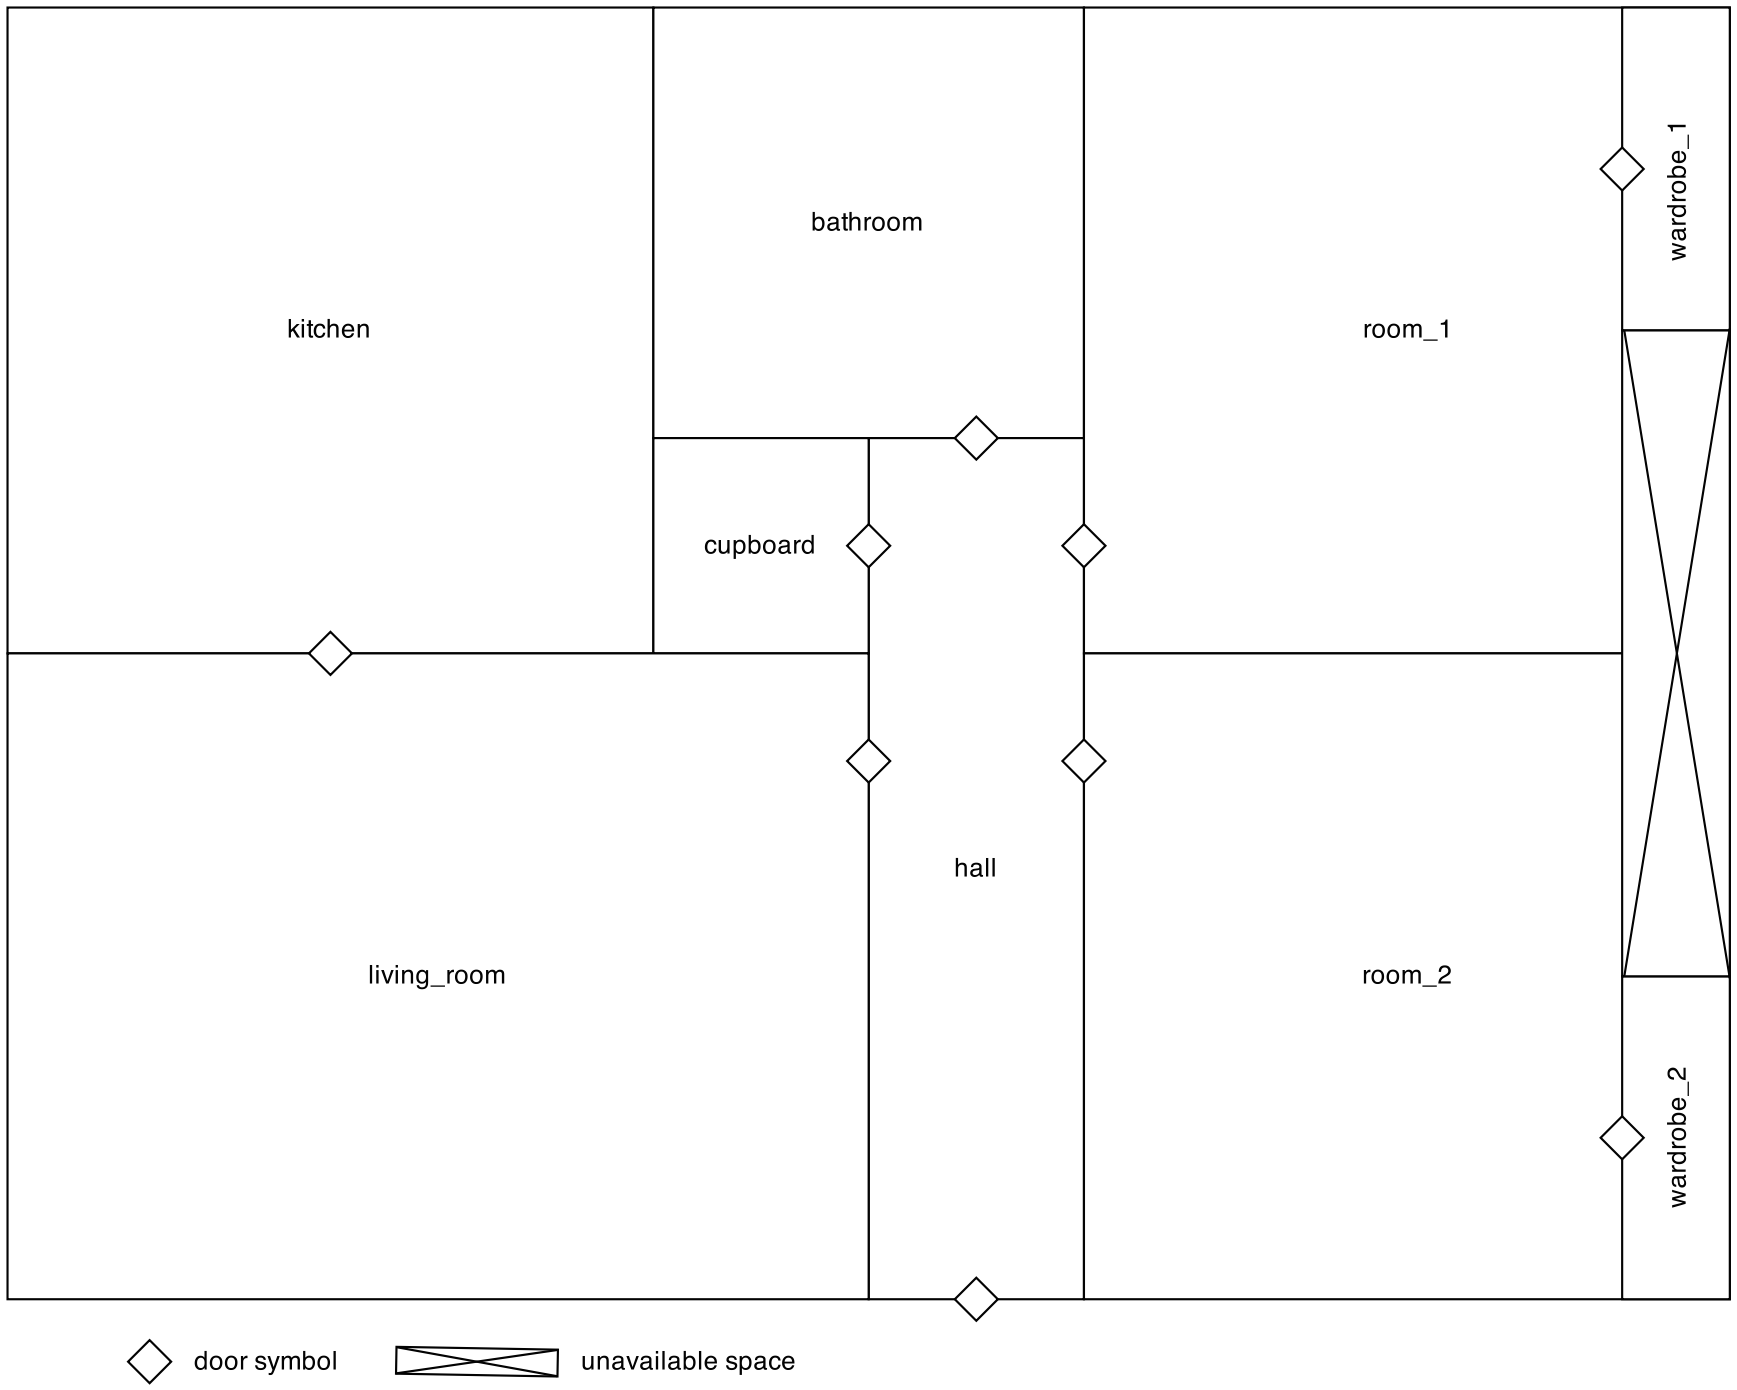
\includegraphics[height=7.3cm]{./gfx/room_layout}
  \caption{Room layout of simulated house.}
\end{figure}

rooms fitted with motion sensors in systematic grid.\\

use coded background knowledge to generate data: sample path and sensor firing\\
tool to generate such data would be of great importance in testing and model building\\

data generator generates smart house data based on 4 description files:
% \section{\texttt{rooms.l}}
Defines interconnection of rooms in form of an adjacency matrix:\\
% \lstinputlisting[language=Python]{../stdg/rooms.l}

The first element in first line must be \texttt{[X]}\\
The headers must be \emph{roomName} --- must be without spaces.

% \section{\texttt{activities.l}}
This file specifies the parameters of Gaussian distribution describing \emph{activities names} in form of:\\
\texttt{nameOfActivity mean standardDeviation}

it is used to simulate time needed to accomplish activity in \emph{seconds}.

% \lstinputlisting[language=Python]{../stdg/activities.l}

% \section{\texttt{path.l}}
This files describe activities to generate in form \texttt{keyword(goal)}:\\
% \lstinputlisting[language=Python]{../stdg/path.l}

the \texttt{keywords} in this file are:\\
\begin{description}
\item[\texttt{start}] where the person starts
\item[\texttt{go}] where to go
\item[\texttt{do}] what activity to do
\end{description}

The \texttt{goals} are:
\begin{description}
\item[room names] defined in \texttt{rooms.l} file and matched with \texttt{go} or \texttt{start} keywords

\item[activities] have to be defined in both \texttt{activities.l} and \texttt{layout.l} files; are matched with \texttt{do} keywords
\end{description}


this file must start with command \texttt{start}\\
to \texttt{do} given activity you first must go to the room that it is available in.

% \section{\texttt{layout.l}}
All measures are in meters\\
the room layout description is based on cartesian coordinates with origin in bottom left corner\\

This file defines sensor layouts for each of the rooms defined in \texttt{rooms.l} file:\\
% \lstinputlisting[language=Python]{../stdg/layout.l}

each room has to be described as:
\texttt{roomName} \texttt{widthOfRoom} \texttt{heightOfRoom} \texttt{:}\\
The room description line has to be finished with \texttt{:}, without spaces.\\

followed by sensors descriptions:\\
\texttt{motionSensorID} \texttt{widthOfSensorLocation} \texttt{heightOfSensorLocation} \texttt{rangeOfSensorRadius}\\
or
\texttt{itemSensorID} \texttt{widthOfSensorLocation} \texttt{heightOfSensorLocation} \texttt{activityName}\\
or\\
door description starting with \texttt{door} keyword and finished with \texttt{roomName} to which the door lead:\\
\texttt{door} \texttt{widthOfSensorLocation} \texttt{heightOfSensorLocation} \texttt{roomName}\\

comment lines start with \texttt{;}\\

    \subsection{Capabilities}
design house
design sensor layout: motion sensor reac

generate arbitrary activities
with ground truth
move arbitrary within the house
prale arbitrary sensors

generate any number of residents

    \subsection{Advantages}

you know whta happens, can design activity structures, get exact ground truth

    \subsection{ILP ready}
----generates background knowledge, positives, negatives, and location activity details
    \subsection{Proof of concept}
--Proof of the generator producing real-life data
Proof for single agent is enough.
Multi agent case is just combination of multiple single agent case with special handling of cases when agents cross each others path i.e. preserving sensor off when someone is inside and double on's and off's\\





  \section{Knowledge representation of spatio-temporal data}
Activity learning method described here requires signals represented as logical facts. ILP system used in this study is written in \texttt{Prolog} programming language therefore, all data has to be expressed in thereof predicates. This requirement causes some problems introduced by sensor type variety.\\

The most common sensor output are binary variables: on-off, present-absent, opened-closed, etc.\ produced by motion and item sensors. Expressing them in predicates is straight-forward as their search space is finite---a set containing two elements.

    \subsection{Unbounded sensor readings}
Another type of sensor output are real and whole numbers. Handling these quantities is well known and broadly documented issue in Artificial Intelligence and Logic Programming. As \texttt{Prolog} is a language based on search space traversal numbers i.e.\ unbounded variables have infinite (unbounded) search space.\\

When sensor output is numerical it is converted to Boolean space by simple shareholding. The critical value is hand-picked based on observation of output values.\\
A special case of unbounded readings is time.

    \subsection{Time representation\label{sec:timeRepresentation}}
Date-time is complex object encoding many useful information. Unfortunately, its human readable format---YYYY-MM-DD HH:mm:SS.ssssss---is of no use in computer science. Converted to machine language it is expressed as a \emph{timestamp}---number of seconds elapsed since epoch dated on 00:00:00, 1\ts{st} January 1970, UTC.\\

For my study I chose to represent time in 4 different way:
\begin{description}
\item[absolute] is timestamp represented in micro-seconds ($\mu$-seconds: $10^{16}s$) rather than seconds,
\item[relative] is number of micro-seconds elapsed since first sensor activation in the dataset,
\item[sequenced] is a sequential number of sensor activation in the dataset starting with $0$,
\item[windowed] is sequential number of fixed-time-interval window that the event fall into; the first time-windows starts on first sensor activation and has ID $0$; window of 5 seconds is used in the study.
\end{description}
Representation examples are shown in \emph{Figure~\ref{lst:timerepresentation}}.\\

\begin{figure}[htb] % [breaklines]
  \begin{minted}[bgcolor=Bkgd,frame=leftline]{Prolog}
sensor(m12, true, relative, 4007842 ).
sensor(m12, true, absolute, 1430004781866056 ).
sensor(m12, true, sequence, 2 ).
sensor(m12, true, windowed, 0 ).

sensor(m13, false, relative, 5994214 ).
sensor(m13, false, absolute, 1430004783852428 ).
sensor(m13, false, sequence, 3 ).
sensor(m13, false, windowed, 1 ).
  \end{minted}
  \caption{Signal represented as \texttt{Prolog} facts.\label{lst:timerepresentation}}
\end{figure}

As no single time representation is best for ILP application all four were tested and evaluated. \emph{Sequence} is most suitable in search space environment---the numbers are not sparse therefore the application can easily iterate through them without large computational overhead.\\
For this reason I chose this representation as the main time format. Despite being helpful in ILP scenario sequential number is highly uninformative. It lacks basic information such as time of day or possibility to be transformed into time elapsed since last sensor reading.\\

To enrich source of information used by learning algorithm \emph{timestamp} representation is used. Following directly from sequence number it can be easily accessed. With such detailed representation of micro-second accuracy, precise time elapsed since any event can be calculated.\\
Moreover this value can be thresholded hence discretised to produce bounded variables such as:
\begin{description}
\item[time of year] winter, summer, autumn, spring;
\item[month] January, February, March, etc.;
\item[time of day] morning, afternoon, evening, night;
\end{description}
and similar. In particular, in ILP and AI such values a lot easier to work with than numbers.\\

The remaining two representations: \emph{relative} and \emph{windowed} are of little use in presented here learning approach.

    \subsection{Background knowledge\label{sec:data:bkg}}
Background knowledge is a general name for a place containing all the information relevant to model learning. By far, it is the most important component of ILP containing building blocks of target model. Moreover, it is a place for logical representation of signals and all relevant rules interacting with them. Additionally, it contains any information not contained or implicit in the raw signals.\\

From large enough sample of smart-house data it is feasible to infer room layout and interconnections, unfortunately this task is computationally complex and impractical in most cases. ILP comes with help in such scenarios as it is ready to use any information not given in raw signals by reading it from background knowledge. Room connections information is great feature as it helps to predict motion trajectory and person's location.\\
Sensor allocation---placement in rooms---is another information not given in raw signal. With help of sensors location, sensor activations can be translated into room name in which the activity is happening.\\
Examples of information used in the background knowledge file is given in \emph{Figure~\ref{lst:bg}}. Fact \texttt{connected\_\_} informs about room connections via doors; \texttt{sensorInRoom} contains information where sensor of given ID is placed; \texttt{sensorActivity} is used with all item and appliance sensors and assigns human readable name to sensor ID; finally, \texttt{sensorInField} tells in range of which motion sensor item or appliance is located.\\

\begin{figure}[htb] % [breaklines]
  \begin{minted}[bgcolor=Bkgd,frame=leftline]{Prolog}
connected__(   bathroom, hall    ).

sensorInRoom(  m61     , bathroom).

sensorActivity(ad1-c   , burner  ).

sensorInField( ad1-b   , m83     ).

aPriori(tv    , watchTV   ).
aPriori(burner, cook      ).
aPriori(phone , phone_call).

bedroom(residentA, bedroom1).
bedroom(residentB, bedroom2).
  \end{minted}
  \caption{Background knowledge facts snippet.\label{lst:bg}}
\end{figure}

Apart from house layout information \emph{prior believes} of any kind can be used in background knowledge---see \texttt{aPriori} keyword \emph{Figure~\ref{lst:bg}}. A priori information such as likely place of activity, device or item required to complete it, and the order of activities are of invaluable help. For example, watching TV is most often associated with living room and a meal cannot be eaten unless it has been cooked. It is a fact that watching television requires TV to be on, cooking is happening on a hob and to make a phone call one needs to use a phone.\\
With multiple residents in a house information such as bedroom assignment helps to distinguish them (\texttt{bedroom} keyword in \emph{Figure~\ref{lst:bg}}).\\

\begin{figure}[htb] % [breaklines]
  \begin{minted}[bgcolor=Bkgd,frame=leftline]{Prolog}
location(Time, Location) :-
  (sensorInRoom(SensorID, Location),
   sensor_state(SensorID, true, Time),
   Time >= 0, !  )
  ;( !, Time > 0,
    location(Time-1, Location) ).
  \end{minted}
  \caption{Example rule.\label{lst:bg:rule}}
\end{figure}

Another component of background knowledge are \texttt{Prolog} rules interacting with facts and signals---they can be understood as \emph{feature extractors}. Rule example is shown in \emph{Figure~\ref{lst:bg:rule}}; it queries \emph{where} (room name) a person is at given \emph{time}.\\

Background knowledge can be also understood as \emph{proxy} between raw signals and high level activity rules. As output rules are based on room, item, appliance names and not sensor IDs they are universal. Already existing model can be applied to any other house by using specific to that place background knowledge.\\
Finally, learnt rules can be used in future iterations of learning process by appending them to the background knowledge.


    \subsection{Positives and negatives\label{sec:data:posneg}}
The final component of ILP are positive and negative examples of model to learn. Sample facts for both single and multiple occupiers are presented respectively in \emph{Figure~\ref{lst:singleposneg}}~\&~\emph{\ref{lst:multiposneg}}.\\

\begin{figure}[htb] % [breaklines]
  \begin{minted}[bgcolor=Bkgd,frame=leftline]{Prolog}
activity(cook  , 47).
activity(eat   , 51).
activity(eat   , 52).
activity(eat   , 53).
activity(washUp, 59).
activity(washUp, 60).
  \end{minted}
  \caption{Positives and negatives for single resident.\label{lst:singleposneg}}
\end{figure}

These examples use \emph{sequence} representation of time to express when (and by whom) activity \emph{is}: positives, and \emph{is not}: negatives done. Both types have common structure and are separated into two different files to be distinguishable.\\

\begin{figure}[htb] % [breaklines]
  \begin{minted}[bgcolor=Bkgd,frame=leftline]{Prolog}
activity(sleep, 14, residentA).
activity(sleep, 15, residentA).
activity(sleep, 16, residentA).
activity(sleep, 17, residentA).
activity(useBathroom, 4, residentB).
activity(useBathroom, 5, residentB).
activity(useBathroom, 6, residentB).
activity(useBathroom, 7, residentB).
  \end{minted}
  \caption{Positives and negatives for multiple resident.\label{lst:multiposneg}}
\end{figure}

For each activity the sets of positive and negative examples have to be disjoint with regard to time. The ILP system generalises positive examples into complex rules containing in body references to sensor states under restriction of not covering any or some negative examples.

  \section{The converter}
The next step in model learning is data conversion from CASAS-like log format to \texttt{Prolog} \emph{knowledge representation} i.e.\ state signal readings as logical facts. The converter is capable of handling both single and multiple residents datasets. To this end, number of conversion steps is need.\\

Real-valued signals like AD1-B water sensor (see \emph{Listing~\ref{lst:CASASoneR}}) are threshold and discretised. Binary sensor output is unified to values \emph{true} and \emph{false}. The time-date information is converted into four described in \emph{Section~\ref{sec:timeRepresentation}} representation.\\
Moreover, the converter uses activity and person ID information given in 4\ts{th} and 5\ts{th} column of the data to generate positive and negative examples needed for learning activity model with \texttt{Aleph}.

  \section{The cross-validation}
Once the data is converted and passed to \texttt{Aleph} the model in form of rules describing activities is produced. To evaluate their quality 10-fold cross-validation is performed.\\
For each script of activities 10 data recordings are gathered together with corresponding model learnt with ILP. Then, each sample model is evaluated on the remaining nine datasets and the results are checked against corresponding ground truth. After testing all possible model-data combinations overall and per-label accuracy and is reported. The output of cross-validation framework is on of the diagnostics used to evaluate model performance.

%===============================================================================
%===============================================================================
%===============================================================================
%===============================================================================
%===============================================================================
\chapter{Inductive Logic Programming\label{ch:ILP}}
\citet{plotkin1972automatic} in early 1970s and \citet{shapiro1983algorithmic} in early 1980s created foundation of \emph{Inductive Logic Programming} (ILP). Both authors introduced techniques and tools to learn \emph{first-order formulas} (parametrised rules that are the core of the ILP) describing chosen object based on a set of facts. Since then, ILP techniques found number of interdisciplinary applications with new tools being created now and then for rules learning purposes.

  \section{Inductive Logic Programming}
The concept of Inductive Logic Programming is based on fusion of two well known techniques: \emph{inductive learning} and \emph{logic programming}. The first component facilitates building model from available observations and generating new knowledge form experience. The latter, introduces a powerful representation of knowledge as \emph{first-order logical rules}~\citep{muggleton1994inductive,muggleton1995inverse}.

    \subsection{Logic programming}
\emph{Propositional logic} widely used in machine learning models is ``\emph{weaker}'' than first-order logic used in ILP. A propositional sentences (rules) are made of facts combined with \emph{logical connectives} such as: not ($\neg$), and ($\land$), or ($\lor$), existence ($\exists$), etc.. Such sentence can only be evaluated to true or false based on predicates in its body e.g.\
$$\left(\left(\texttt{sensorM42} \land \texttt{sensorM47}\right) \lor \left(\texttt{sensorM27} \land \texttt{sensorM30}\right)\right) \land time = 40$$
where \texttt{sensor$\Bigcdot\Bigcdot\Bigcdot$} denotes sensor $\Bigcdot\Bigcdot\Bigcdot$ being on, is true if either both \texttt{sensorM42} and \texttt{sensorM47} or \texttt{sensorM27} and \texttt{sensorM30} are simultaneously on at time $40$.\\

Thanks to first-order logic ILP overcomes mentioned above ``limited representation formalism'' (expressing data in form of a propositional logic). Many problems considered hard to solve while expressed propositionally can be easily tackled with ILP. The power of first-order logic lies in expressing its sentences with \emph{parametrised} predicates. Use of domain specific quantified variables alters logical state of sentence based on their input and output therefore facilitates expressing complex relations. An example of first-order activity rule: \texttt{activity(A,B)} where variable \texttt{A} denotes activity ID and \texttt{B} time, is given below. The rule illustrates the dependence between predicates via free variables.\\
\begin{eqnarray*}
&\texttt{activityOrder(B,A)} \land \texttt{location(B,livingRoom)} \land \\
&\texttt{outOfCabinet(B,C)} \land \texttt{medicineInList(C)}
\end{eqnarray*}
The major limitation of first-order logic is its restriction to finite variable domains---it cannot describe rules built on infinite sets like real or natural numbers.\\

Finally, ILP does not have difficulties in incorporating substantial background knowledge in form of first-order sentences to the model. This feature is not very common among machine learning models, nevertheless, use of domain knowledge is ``essential for intelligent behaviour''~\citep{muggleton1994inductive}.

    \subsection{Inductive learning}
The second component of ILP is inductive learning: constructing \emph{first-order clausal theories}. Such hypotheses are based on combining background knowledge with facts representation of positive and negative examples; see \emph{Figure~\ref{fig:ilp}}.\\
\begin{figure}[htb]
  \centering
  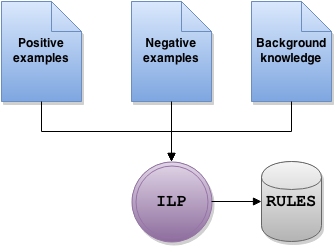
\includegraphics[scale=.5]{./gfx/ilp}
  \caption{ILP scheme\label{fig:ilp}}
\end{figure}
ILP aims at building theory that under consideration of background knowledge explains facts: covers as much positive examples as possible without covering and or most of negative examples. To this end, it uses \emph{induction} as a basic mode of inference: generalization of specific observations to theories, rather than deduction: transforming general theories to the more specific clauses.

    \subsection{Applications}
The rules produced with ILP are human readable unlike models produced by majority of machine learning solutions, what gives it great advantage over competition. Easy to understand rules means that the logic models are arguably easy to manipulate. They can be changed by simply adding, deleting, and modifying clauses or literals.\\
Such model representation is invaluable in \emph{scientific theory formation} and problems where data cannot be easily represented in attribute-vale language. ILP is widely used in structure-activity prediction for drug design~\citep{king1992drug,michael1992modelling} and protein secondary-structure prediction~\citep{muggleton1992protein}. It is also popular tool in computer science as: programming assistance, algorithmic debugging, program testing and verification, and reverse engineering~\citep{shapiro1983algorithmic,bergadno1993inductive,bratko1993inductive}.\\

The two most popular \texttt{Prolog} ILP implementations are \texttt{Aleph}\footnote{\url{http://www.cs.ox.ac.uk/activities/machlearn/Aleph/aleph.html}} and \texttt{Progol}\footnote{\url{http://www.doc.ic.ac.uk/~shm/progol.html}}. \texttt{Aleph} is chosen for this study due to its comprehensive documentation availability and ease of use on contemporary platforms.

  \section{\texttt{Aleph}}
\texttt{Aleph}: A Learning Engine for Proposing Hypotheses, is \texttt{Prolog} based Inductive Logic Programming system developed at Oxford University by \citeauthor{muggleton1994inductive}. It is compatible with two most popular \texttt{Prolog} language implementations: \texttt{YAP}---Yet Another Prolog, and \texttt{SWI-Prolog}.

    \subsection{Input files}
\texttt{Aleph} infers hypotheses using three files, the first two contain positive and negative examples of target rule model, the third encodes program settings and additional informations.

      \subsubsection{Background}
Background file contains \texttt{Aleph} configuration and target model specification; see example given in \emph{Figure~\ref{lst:alephSettings}}. Settings such as used evaluation function, allowed maximal number of negative examples covered by a single target rule, and minimal number of positive examples that each rule has to cover are used.\\
Additionally, user provides target rule specification. Based on presented example the target \texttt{activity} rule has $2$ variables (is of \emph{arity} $2$): (constant, \#) activity ID and (input, +) integer representing time. The body of the rule can contain arbitrary number of \texttt{device} and \texttt{location} predicates each having $2$ variables. The first takes integer time input and constant device ID; the latter integer time input and constant room ID.\\
Finally, target model constrains can be specified (\texttt{false} keyword): in presented example no two activities can happen at the same time.\\
\begin{figure}[htb] % [breaklines]
  \begin{minted}[bgcolor=Bkgd,frame=leftline]{Prolog}
% Internal settings
:- set(evalfn, wracc).
:- set(noise , 3    ).
:- set(minpos, 1    ).
% Determinations
:- determination(activity/2, device/2  ).
:- determination(activity/2, location/2).
% Mode declarations: rule head definition
:- modeh(*, activity(#activityIDs, +integer) ).
% Rule body definition
:- modeb(*, device(+integer, #deviceIDs)).
:- modeb(*, location(+integer, #roomIDs)).
% Constrains
false :-
  activity(Activity1, T),
  activity(Activity2, T),
  not(Activity1 = Activity2).
  \end{minted}
  \caption{Example \texttt{Aleph} settings.\label{lst:alephSettings}}
\end{figure}
Therefore, target rules are of the form \texttt{activity(ActivityID, Time) :- $\Bigcdot$}.\\

Additionally to presented above \texttt{Aleph} settings, background knowledge file also contains facts and rules discussed is \emph{Section~\ref{sec:data:bkg}}.

      \subsubsection{Positives}
Positive examples file lists activity facts of the form \texttt{activity(ActivityID, Time).} to indicate at which time points the activity was happening in a data. Example file is discussed in \emph{Section~\ref{sec:data:posneg}}.

      \subsubsection{Negatives}
Negative examples file is of the same form as positive example file. It indicates time-points when activities were not undertaken. In presented here learning scenario the negative time-points are set complement of positives examples and are bounded from below by $0$ and from above by number of sensor readings in the data set; see \emph{Figure~\ref{fig:timepoints}} for reference. Example file is discussed in \emph{Section~\ref{sec:data:posneg}}.
\begin{figure}[htb]
  \centering
  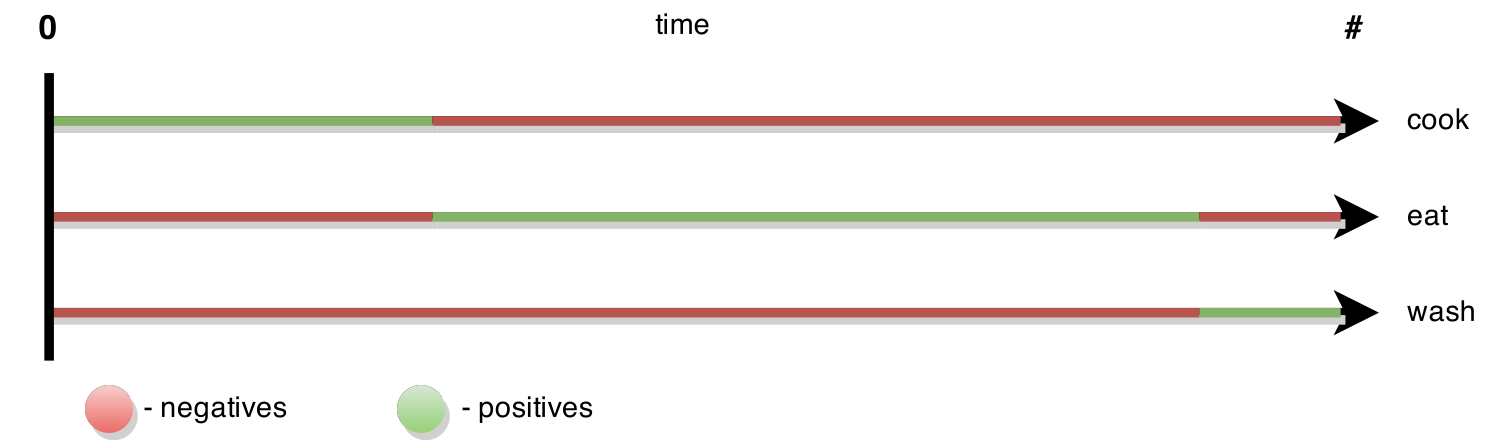
\includegraphics[width=.85\textwidth]{./gfx/activityStructure}
  \caption{Activity structure example.\label{fig:timepoints}}
\end{figure}

    \subsection{\texttt{Aleph} output}
Based on input data \texttt{Aleph} outputs set of rules compliant with given specification. Presented in \emph{Figure~\ref{lst:alephSettings}} settings could result in first from the top rule given in \emph{Figure~\ref{lst:alephOut}}. It does not contain free variables in the body hence can be expressed in propositional logic.\\
The second one is more complex yet still propositional. \texttt{outOfCabinet(A,[none])} predicate gives list of items taken out of cupboard at time \texttt{A}.\\
The third activity rule is a \emph{singularity}. Positive example \texttt{activity(clean,87).} is outputted as the ILP algorithm could not generalised it to proper rule without breaking any of the restrictions imposed by the background file. Such rules are pruned out prior to cross-validation.\\
\begin{figure}[htb] % [breaklines]
  \begin{minted}[bgcolor=Bkgd,frame=leftline]{Prolog}
activity(wash_hands,A) :-
  device(A,water_hot).

activity(wash_hands,A) :-
  outOfCabinet(A,[none]),
  waterUsed(A).

activity(clean,87).
  \end{minted}
  \caption{Example activity model.\label{lst:alephOut}}
\end{figure}

An example of more advanced, first-order logical rule is presented in \emph{Figure~\ref{lst:bg:rule}}. Free variables present in the rule body ensure clauses interaction.

    \subsection{The basic algorithm}
Generally speaking, inductive logic programming is a \emph{search problem}. The algorithm traverses through \emph{candidate solution space} i.e.\ set of ``well-formed'' hypotheses, to find the most suitable one. ILP problem can be solved using na\"{\i}ve generate and test algorithm however, this approach is highly inefficient. The most suitable solution has four steps: select example, build most-specific-clause, search, and remove redundancies~\citep{muggleton1994inductive}.

      \subsubsection{Select example}
Select positive example that is not yet covered by learnt rule form the positives set. If all were tested stop the procedure.

      \subsubsection{Build most-specific-clause}
Also known as \emph{saturation step}. Construct \emph{bottom clause}: definite clause with many literals that is most specific given that it entails previously selected example and complies with provided restrictions.

      \subsubsection{Search}
Also known as \emph{reduction step}. Search through subsets of previously found literals to build more general clause .
for improved performance

      \subsubsection{Remove redundancies}
The clause with the best score is added to the current theory, and all examples made redundant are removed. This step is sometimes called the "cover removal" step. Note here that the best clause may make clauses other than the examples redundant. Again, this is ignored here. Return to Step 1.\\
remove clauses not imporveing classification results to become more general -> better for prediction\\
repeat

  \section{Applications to spatio-temporal data}
built with events, where each event is based on sensor readings
pros and cons
Use of background knowledge
failure by negation -> if we don't know whether it;s on -> it's not
easy meta-rule writing adn fixing continuity issues

  \section{Closed Concept \& Least General Generalisation}
ILP reduces the result.
activity description
keep not needed clauses in body.

``A closed concept is a concept where all the necessary and sufficient conditions required to include something within the concept can be listed. For example, the concept of a triangle is closed because a three-sided polygon, and only a three-sided polygon, is a triangle. All the conditions required to call something a triangle can be, and are, listed.''

  \section{Feature discovery and feature extraction}
Rules used in a body of activity rules can be understood as features.
Therefore they can be as well extracted and used with other models

Name the most popular that I use


%===============================================================================
%===============================================================================
%===============================================================================
%===============================================================================
%===============================================================================
\chapter{Sequential multi-class model---single resident\label{ch:smcm}}
presented above example both \texttt{location} and \texttt{device} rules can be transformed to become features. Rebuilt dataset may become more ``informative'' than the original one, therefore, it can improve classification carried out with variety of different machine learning models.

  \section{Evaluation measures}
  \section{Simple synthetic dataset}

Example of ILP rules learnt with \texttt{Prolog} are shown in \emph{Listing~\ref{lst:eg}}.

  \section{Synthetic CASAS \#2}
narrated datasets
  \section{CASAS \#2}
narrated datasets
  \section{Discontinuity}
Continuity rule --- introducing bias\\
Meta-rule -- smoothing out predictions
  \section{Model generality}
Generality of learnt rules (synthetic <--> genuine) Results overview
  \section{Overlapping activities}
single resident multi-label case

  \section{Features}


% \vspace{1em}
% \begin{figure}[htb]
% \lstset{
%   captionpos=b,
%   frame=single,
%   language=Prolog,
%   breaklines=true,
%   caption=Example of target rules.,
%   label=lst:eg,
%   float=tb
% }
% \begin{lstlisting}
\begin{figure}[htb] % [breaklines]
  \begin{minted}[bgcolor=Bkgd,frame=leftline]{Prolog}
activity(Person, cooking) :-
  location(Person, TimeWindow, kitchen), device(TimeWindow, hob).
activity(Person, watchingTV) :-
  location(Person, TimeWindow, livingRoom), device(TimeWindow, tv).

location(Person, TimeWindow, kitchen) :-
  sensor(1, on, TimeWindow), sensor(5, on, TimeWindow).
location(Person, TimeWindow, livingRoom) :-
  sensor(2, on, TimeWindow), sensor(7, on, TimeWindow).

device(TimeWindow, hob) :-
  sensor(101, on, TimeWindow).
device(TimeWindow, tv) :-
  sensor(105, on, TimeWindow).
  \end{minted}
  \caption{Caption.\label{lst:label}}
\end{figure}
% \end{lstlisting}
% \end{figure}





%===============================================================================
%===============================================================================
%===============================================================================
%===============================================================================
%===============================================================================
\chapter{Multi-label model---multiple residents\label{ch:mlm}}
  \section{Evaluation measures}
  \section{Bathroom excursion}
    \subsection{Movement case}
    \subsection{Still case}

  \section{CASAS \#9}

  \section{Features}


%===============================================================================
%===============================================================================
%===============================================================================
%===============================================================================
%===============================================================================
\chapter{Summary\label{ch:summary}}
generally about what i've done

  \section{Smart-house data generator}
Data generator as a helpful tool for building and testing models\\

  \section{Rule based Activity Recognition Model}
ILP can be used as one of models for activity recognition: its strong points not available (or hard to achieve) in other models

  \section{Work evaluation}
what my results mean to general public

  \section{Further development: Data Narrative\label{sec:narrative}}

Proposed here ILP tool could extend suit of available analytic technologies for activity recognition and become great foundation for \emph{Narrative Analtics} presented in \emph{Section~\ref{sec:narrative}}.

Proposed here rules learning mechanism can be extended with ``grammar'' capable of generating \emph{Narrative Analysis} of spatio-temporal data: a \emph{succinct natural language description} of a selected time-space window of the data of interest. In healthcare and smart house scenarios, such techniques can be combined with activity recognition models to generate comprehensible descriptions of monitored activities with terminology and level of detail tuned to a particular recipient. In the context of the SPHERE project these techniques would facilitate making sense from acquired data for healthcare applications in a more transparent way than is possible with black-box approaches.

Human activities can be hierarchically organised with complex actions composed of sub-actions, until ``atomic level'' is reached. This creates possibility to apply filters to produce multiple levels of narrative complexity based on target audience. Adjusting level of detail (granularity) of produced description would result in emphasis on different aspects of carried out activities during period of interest, hence, extracting relevant for the audience information.\\

    \subsection{Visualisation techniques}
Most commonly used visualisation techniques nowadays are tables, graphs, and diagrams. Unfortunately, such charts often need expertise in a field to be correctly interpreted. Moreover, aforementioned methods often trade-off clarity for completeness of shown data hence make it difficult for a broad audience to see the big picture.\\

\emph{Narrative Analysis} aims at exploring possibility of describing data with natural language. This form of expressing information contained in the data has been under-appreciated and devoted little attention in recent years. Deep learning techniques have been applied to images to generate succinct scene description, nevertheless, it has not been used with raw data.\\
An example of data narration can be found in modern smart-phone weather and calendar applications where instead of detailed weather forecast or hour-by-hour calendar events, one sentence description is presented to the user. Furthermore, in recent years \emph{narrative analytics} in combination with visualisation techniques have been proven as effective method of expressing corporate financial data.\\

Successful adaptation of \emph{Narrative Analytics} to data provided by smart houses would greatly benefit healthcare applications. Being able to deliver activity description within given time-space window and with different level of detail would provide invaluable monitoring and diagnostic tool for daily care personnel and medical staff.

    \subsection{Narrative Analytics}
Presented here extension is not restricted to smart house data. \emph{Narrative Analytics} can be applied to any spatio-temporal information---e.g.\ smart-city feed---resulting in brief situation description contained in the data. Such ``label'' gives possibility to quickly understand status of the system without time-consuming raw-data or charts interpretation. Improved response time would result in appropriate actions taken instantly, whether it is better disease diagnosis, or traffic conditions displayed in timely manner on interactive information signs.\\
Moreover, as produced description would also be hierarchical it can be formed in a ``tree'' structure with more general narratives being higher in hierarchy. Creating timetable filled with activity ``labels'' would give better insight into personal habits and routines yielding improved understanding of arising issues.\\
Furthermore, proposed here descriptive mechanisms could be extended to become a query-enabled database. In such model a user could ``ask'' a question in natural language to get narrative answer instead of numerical vector.\\

Data narration can have multiple other applications. Alternatively, it can be used to produce figure caption based on data used to draw it.

% challenges
Creating a narrative of events is composed of two major components---``grammars'' needed to transform the data: \emph{data analysis}(objective of this project) and \emph{narrative generation}.\\
The first one is deriving high-level knowledge from low-level data (sensor input) with ILP. The latter is ``translating'' extracted information into natural language description, which also can be done using similar approach.


\begin{center}
\noindent \line(1,0){250}
\end{center}

\bibliography{yhpargoil}{}
\bibliographystyle{plainnat}
% \bibliographystyle{plain}

\end{document}

% useful expressions:
%% aggregate signal
% \citeauthor{BiBTeX_reference}
%  as opposed to
